\section{Overview of the Code Generation Flow}
We leverage the \MLIR compiler infrastructure.
\MLIR drastically reduces the entry cost to define, compose and reuse abstractions for the construction of domain-specific compilers.
It offers a comprehensive collection of solutions to compiler construction challenges by:
(1) standardizing Static Single Assignment (SSA) form representations and data structures,
(2) unifying compiler analyses and transformations across semantic domains through generic programming concepts such as operation traits and interfaces,
(3) providing a declarative system for defining operations with nested regions, and domain-specific type systems, and
(4) providing a wide range of services including documentation, parsing/printing logic, location tracking, multithreaded compilation, pass management, etc.

\MLIR is designed around the principles of parsimony, progressivity and traceability~\cite{lattner2021mlir}. 
The code generation approach presented in this paper has largely contributed to the establishment of these principles and actively leverages them. 
The internal representation in \MLIR is fully extensible, allowing for custom user-defined operations (instructions), attributes and types. 
IR components that are expected to work together are grouped into \emph{dialects}, which can be seen as the intermediate representation analog of dynamic libraries. 
Unlike many earlier compilation flows that have multi-level yet all-or-nothing internal representation, \MLIR affords and encourages the mix of different dialects in a single unit of compilation at any point in the compilation flow. 
For example, a high-level tensor product operation may co-exist with low-level hardware instructions on vector elements in the same function. This provides a great level of modularity, composition and optionality that makes it possible to use the right abstractions for solving a particular problem, \emph{instead of having to solve all problems in a unique  representation}.

\subsection{Bird's Eye View and Motivation of Structured and Retargetable Code Generation}

Code generation approaches for numerical computing have traditionally focused on optimizing the performance of loop nests. 
Associated analyses focus on scalar elements as the body of a loop nest typically computes a single element. 
Such analyses must consider memory dependences and aliasing. 
These approaches have been deeply researched in the past~\cite{AllenKennedy} and have reached a high level of maturity. 
They are well-suited when starting from an input language like C or Fortran where the problem is already specified in terms of loops over data residing in pre-allocated memory.

When focusing on a specific domain (e.g.\ the ML space), we have the luxury of programs defined at a much higher level of abstraction than loops. 
This opens up the opportunity to revisit classical loop optimizations like fusion, tiling or vectorization without the need for complicated analysis and heuristics.
Advantages include reduced complexity and maintenance cost while also scaling naturally to extensions like sparse tensors, that are even more difficult to analyze at the loop level.

It makes it possible to avoid raising information from lower level representations by means of static analysis, where feasible, and performing optimizations at the highest possible level of abstraction.
We refer to this approach as \emph{structured code generation} since the compiler primarily leverages structural information readily available in the source code. 
Figure~\ref{fig:birds-eye-view-of-structured-codegen} shows a coarse-grained summary structure of the steps and levels of abstraction involved.

The starting point (Structured IR) is composed of tensor algebra operations, organized as a functional program over dense and sparse tensors.

\begin{figure}[h!tb]
\centerline{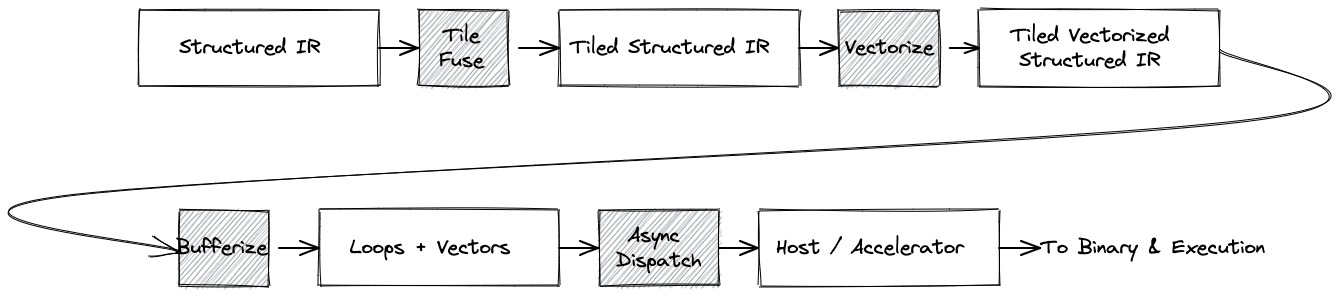
\includegraphics[width=14cm]{figures/BirdsEyesViewCodegenFlow.png}}
\caption{\label{fig:birds-eye-view-of-structured-codegen}Bird's eye view of structured and retargetable code generation.}
\end{figure}

From this level we move to a tiled structured level, which introduces loops by tiling the operations. 
Multiple, gradual tiling steps are possible, and do not necessarily result in loops around scalars. 
Instead, tiling produces loops around structured operations similar to the original ones but on smaller tensors. 
We also perform fusion of tensor operations at this level. 
The final granularity of operations is chosen to make their hardware mapping efficient.
A prototypical example is to tile a matrix multiplication to model the cache hierarchy and then lower the smaller matrix multiplication directly to a superoptimized microkernel in assembly language.

In the next step, we map computations on resulting small tensors to a (retargetable) vector abstraction. 
This mapping exploits high-level knowledge about the operations that we have carefully preserved. 
In particular, it is not required to analyze the loop control flow enclosing the finer-grained tensor operations. 
This step might also include enabling transformations like padding for efficient cache access free of cache-line splitting and vectorization.

What makes \emph{structured code generation} highly composable and reusable is that tiling and fusion transformations are both fully generic in the operations and data types they operate upon. 
These transformations only assume a generic, monotonic (from the point of set inclusion), structural decomposition pattern associated with computations and composite data. 
Both dense and sparse tensor algebra exhibit such blockwise decomposition patterns, and the code generation abstractions and infrastructure generically applies to both.
This is also true of future computations and data structures following the same pattern.

Up until now, computations took place on immutable tensor values. 
We lower this to a representation on side-effecting buffers in the next step. 
This results in a representation with nested loops on vectors and side-effects.
More optimizations on loops and memory accesses happen at this level.

In the final step, we may translate the representation directly to the \lstinline|llvm| dialect of \MLIR for sequential execution on CPU, or offload a GPU kernel, or split up loops into \lstinline|async| blocks for a task parallel runtime, etc.

This flow composes with existing affine analyses and loop optimizations as implemented in \MLIR, and that have been largely explored in the literature.
In fact, the packing and loop peeling transformations in our flow leverage and helped generalize the MLIR affine machinery.

While this flow is but a first stake in the ground, it already demonstrates how to achieve a modular and composable system.
It is also built with optionality in mind: for some operations, skipping levels or even a fully divergent flow are viable options.
This is made possible by our work establishing the \emph{progressive lowering principle}: every step is materialized in the IR and very little load-bearing logic is abstracted away from the user (e.g.\ in the form of complex C++ logic deep inside the compiler implementation of analyses and heuristics).
We expect more operations and data types will be designed and implemented that do not fit the current code generation stack of abstractions.
While this allows to extend the structured and progressive lowering approach to other application domains, we acknowledge that not all computations in ML or HPC will necessarily be covered by the current approach, alone.
This is where composability, modularity and optionality kick in: \emph{not all problems need to be solved in the same abstraction, rather we should use the best abstraction for each different classes of problems}.

\subsection{Short Introduction to MLIR}

\begin{figure}
  \centering
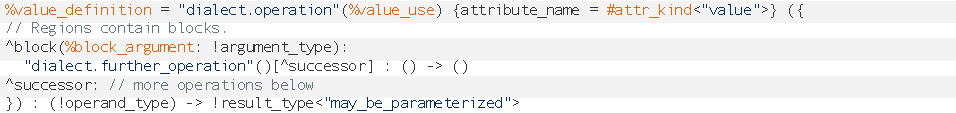
\includegraphics[width=\textwidth]{figures/mlir_example_large}
  \caption{\MLIR concepts in the generic format. \MLIR has an open set of attributes, operations and types. Operations may recursively contain regions of blocks with further operations.}
  \label{fig:mlir_concepts}
\end{figure}

The \MLIR infrastructure builds on the success of \LLVM~IR while providing unprecedented extensibility.
\MLIR has an open, easily extensible set of instructions, called \emph{operations} that typically represent the dynamic semantics of the program.
Operations can represent anything from hardware instructions, or even hardware itself, to building blocks for machine learning models such as layers or blocks thereof.
They define and use values, which represent units of immutable data in SSA form.
The compile-time knowledge about values is captured in \emph{types}, and the knowledge about operations is captured in \emph{attributes}.
Attribute and type systems are similarly open and extensible.
IR objects can be logically grouped together in libraries, called \emph{dialects}.
The \MLIR~IR has a recursive structure where operations may have additional \emph{regions} containing a graph of (basic) \emph{blocks}, which in turn contain further operations. Figure~\ref{fig:mlir_concepts} illustrates key \MLIR concepts.

In addition to common components such as the compiler pass infrastructure, \MLIR provides tools to manage its extensibility, many of which evolved or were specifically designed to support the code generation flow presented in this document. In particular, \MLIR features attribute, operation and type \emph{interfaces} similar to object-oriented programming languages allowing one to work with abstract properties rather than (fixed) lists of supported concepts. Interfaces can be implemented separately from operations, and mixed in using \MLIR's registration mechanism, thus fully separating IR concepts from transformations.

\subsection{Dialects Relevant to Code Generation}
\label{subsec:dialects-relevant-to-code-generation}

The domain-specific abstractions we design and implement comprise representations for the following dialects, listed in increasing level of abstraction.
Following our modularity and optionality design principles, any of these dialects can be mixed with others or simply bypassed if it does not provide a useful abstraction for a particular case.

\subsubsection{\lstinline|vector| Dialect}
\label{sec:vector-dialect}

This dialect provides a fixed-rank \emph{n-D} vector type, e.g., \lstinline|vector<4x3x8xf32>|, as well as operations that form an intuitive and retargetable \emph{vector programming model} that conceptually extends the traditional 1-D vector instructions to arbitrary rank.
Such operations can decompose progressively into lower-rank variants of themselves. They further lower to \LLVM vector instructions (e.g.\ \lstinline|shufflevector|) when the backend heuristics are robust enough to generate near-peak assembly or bypass that level and directly target hardware-specific intrinsics (e.g.\ \lstinline{gpu.subgroup_mma_compute_matrix} 2-D vector instructions or \lstinline{amx.tile_mulf} 2-D tile instructions).

\subsubsection{\lstinline{gpu} Dialect}

The \lstinline{gpu} dialect defines the retargetable \emph{GPU programming model}.
It features abstractions common to SIMT platforms, such as the host/device code separation, workitem/group (thread/block) execution model, communication and synchronization primitives, etc.
This dialect can be produced from the \lstinline{vector} dialect and can itself be lowered to platform-specific dialects such as \lstinline{nvvm}, \lstinline{rocdl} or \lstinline{spirv}.
It is only listed to illustrate the overall retargetability of our approach and is not discussed further in the paper.

\subsubsection{\lstinline|memref| Dialect}

The \lstinline|memref| dialect introduces the \lstinline|memref| data type, which is the main representation for \emph{n-D} memory buffers in \MLIR and the entry point to the side-effecting memory-based operations, and the operations to manage buffer allocation, aliasing (memref \emph{views}) and access.
Unlike traditional pointers, \lstinline|memref|s are multi-dimensional buffers with explicit layout that allows for decoupling the indexing scheme from the underlying storage: \lstinline|memref<10x10xf32, strides: [1,10]>| affords column-major access while having row-major storage.
The \lstinline|memref| data type also provides an unsurprising ABI to interoperate with external C code, useful to interact with libraries.

\subsubsection{\lstinline|tensor| Dialect}
\label{subsubsec:tensor-dialect}
The tensor dialect operates on an abstract n-D tensor type for which we have not yet decided on a representation in memory. 
During the compilation, sufficiently small tensors of static sizes may be placed directly in (vector) registers while larger or dynamically-sized tensors are put into memory storage thanks to the bufferization process.
Tensor values are \emph{immutable} and subject to def-use SSA semantics, operations on tensors are often free of side-effects.
This allows classical compiler transformations such as peephole optimizations, constant subexpression and dead code elimination, or loop-invariant code motion to apply seamlessly to tensor operations regardless of their underlying complexity.
\emph{Since tensor values are immutable, they cannot be written into. Instead, ``value insertion'' operations create new tensors with a value or a subset thereof replaced.}
\footnote{This is analogous to the design of \texttt{struct} in LLVM IR:
\texttt{\%1 = insertvalue \{f64, f32, i32\} \%0, f32 42.0, 1} defines a new value \texttt{\%1} that holds the same elements as \texttt{\%0} except for the element at position \texttt{1} that now holds \texttt{42.0}.
}

\subsubsection{\lstinline|scf| Dialect}
The \emph{structured control flow} \lstinline|scf| dialect provides operations that represent looping and conditionals (e.g.\ regular \lstinline|scf.for| and \lstinline|scf.while| loops without early exit as well as an \lstinline|scf.if| conditional construct) and \emph{embeds them into the SSA+regions form} of \MLIR.
This is structured at a higher-level of abstraction than a control flow graph. Notably, \lstinline|scf| loop operations may yield SSA values and compose well with other operations and dialects with either memory-based side-effecting semantics or SSA-based side-effect-free semantics.

\subsubsection{\lstinline|linalg| Dialect}
The linalg dialect provides higher-level compute primitives that can operate on both \lstinline|tensor| and \lstinline|memref| containers. These primitives can decompose into versions of themselves operating on structured \emph{subsets} of the original input data and producing similarly structured subset of their results. They also capture program invariants and structural information, such as independency of certain parts of computation or reduction patterns, that decreases the need for expensive analyses prior to transformation.

\subsubsection{\lstinline{sparse_tensor} Dialect}
The sparse tensor dialect provides the types and transformations required to make sparse tensor types first-class citizens within the MLIR compiler infrastructure. The dialect bridges high-level \lstinline|linalg| that operates on sparse tensors with lower-level operations on the actual sparse storage schemes that save memory and avoid performing redundant work.

\subsection{Lower-level Dialects: Producing LLVM IR and Binaries}
\begin{figure}[h!tb]
\centerline{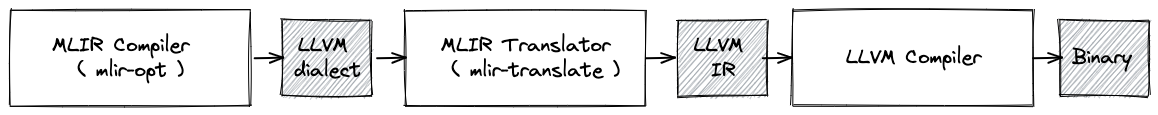
\includegraphics[width=14cm]{figures/MLIRtoLLVM.png}}
\centerline{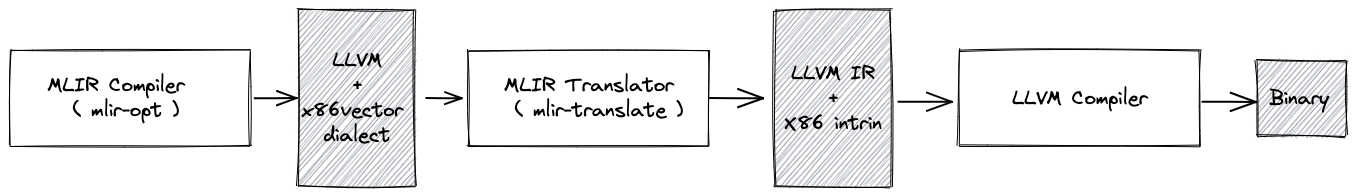
\includegraphics[width=14cm]{figures/MLIRtoLLVMandIntrinsics.png}}
\caption{Simple visual description of the MLIR compiler flow: (top) \texttt{llvm} dialect only, (bottom) \texttt{llvm} and \texttt{x86vector} dialects, the latter containing hardware-specific ``intrinsic'' operations.}
\label{fig:simple-mlir-flow}
\end{figure}

At the end of the transformation process, \MLIR produces low-level dialects common to multiple compilation paths.
The \lstinline|llvm| dialect closely mirrors \LLVM IR and is the output we consider in this paper.
The \MLIR module using this dialect can be \emph{translated} to \LLVM IR before being handed off to the \LLVM compiler to produce machine code.
Figure~\ref{fig:simple-mlir-flow}(top) summarizes the tool flow.

Similarly to the rest of \MLIR, this dialect can be mixed with other ones.
In particular, it reuses built-in \MLIR types such as integer (\lstinline{i32}) or floating-point (\lstinline{f32}) scalars.
A detailed example of such a dialect mix is discussed in Appendix~\ref{sec:appendix-llvm-mix-example}.

While our flow mostly relies on the \LLVM compiler to perform common middle-end and back-end optimizations, some performance-critical scenarios require stronger guarantees of specific hardware instructions being emitted.
Therefore \MLIR provides a handful of low-level platform-specific dialects: \texttt{nvvm}, \texttt{rocdl}, \texttt{x86vector}, \texttt{arm\_neon}, \texttt{arm\_sve}, \texttt{amx}, etc.
These dialects partly mirror the corresponding sets of \LLVM IR intrinsic functions, which themselves typically map to hardware instructions.
Beyond making these instructions first-class operations and providing, these dialects also define slightly higher-level operations that make use of \MLIR's extensible type system and other capabilities.
For example, the
\begin{lstlisting}[language=mlir]
arm_neon.2d.sdot : vector<4x4xi8>, vector<4x4xi8> to vector<4xi32>
\end{lstlisting}
operation is naturally expressed on a \MLIR multidimensional vector type.
Before converting to \LLVM IR, it is first lowered to
\begin{lstlisting}[language=mlir]
arm_neon.intr.sdot : vector<16xi8>, vector<16xi8> to vector<4xi32>
\end{lstlisting}
that operates on flattened 1-D vectors to match \LLVM's convention.
The full example is provided in Appendix~\ref{sec:appendix-arm-neon-example}.
